\documentclass[listings]{labreport}
\usepackage{amsmath}
\usepackage{geometry}
\usepackage{array}
\subject{Теория автоматов}
\titleparts{Практическое задание №3}{Вариант 8}
\students{Лабушев Тимофей}
\usepackage{caption}
\captionsetup{justification=raggedright, singlelinecheck=false}

\begin{document}

\maketitlepage

\section*{Цель работы}

Практическое освоение метода перехода от абстрактного автомата
к структурному автомату.

\section*{Задание}

Абстрактный автомат задан табличным способом. Причем абстрактный автомат Мили
представлен таблицами переходов и выходов, а абстрактный автомат Мура — одной
отмеченной таблицей переходов. Для синтеза структурного автомата использовать
функционально полную систему логических элементов И, ИЛИ, НЕ и автомат Мура,
обладающий полнотой переходов и полнотой выходов. Синтезированный структурный
автомат представить в виде ПАМЯТИ и КОМБИНАЦИОННОЙ СХЕМЫ.

\section*{Исходный автомат Мили}

\begin{tabular}{|*{7}{c|}}
\hline
$\delta$ & $a_1$ & $a_2$ & $a_3$ & $a_4$ & $a_5$ & $a_6$\\\hline
$z_1$ & $a_2$ & $a_1$ & $a_5$ & $a_6$ & $a_2$ & $a_3$\\\hline
$z_2$ & $a_4$ & $a_3$ & $a_1$ & $a_4$ & $a_6$ & $a_5$\\\hline
$z_3$ & $a_6$ & $a_5$ & $a_3$ & $a_2$ & $a_4$ & $a_1$\\\hline
\end{tabular}
\begin{tabular}{|*{7}{c|}}
\hline
$\lambda$ & $a_1$ & $a_2$ & $a_3$ & $a_4$ & $a_5$ & $a_6$\\\hline
$z_1$ & $w_1$ & $w_2$ & $w_3$ & $w_3$ & $w_2$ & $w_1$\\\hline
$z_2$ & $w_2$ & $w_3$ & $w_1$ & $w_2$ & $w_1$ & $w_3$\\\hline
$z_3$ & $w_3$ & $w_1$ & $w_2$ & $w_1$ & $w_3$ & $w_2$\\\hline
\end{tabular}

\section*{Двоичное кодирование исходного автомата}

Входной алфавит:

\begin{tabular}{|*{3}{c|}}
\hline
$$ & $x_1$ & $x_2$\\\hline
$z_1$ & $0$ & $0$\\\hline
$z_2$ & $0$ & $1$\\\hline
$z_3$ & $1$ & $0$\\\hline
\end{tabular}

Выходной алфавит:

\begin{tabular}{|*{3}{c|}}
\hline
$$ & $y_1$ & $y_2$\\\hline
$w_1$ & $0$ & $0$\\\hline
$w_2$ & $0$ & $1$\\\hline
$w_3$ & $1$ & $0$\\\hline
\end{tabular}

Состояния:

\begin{tabular}{|*{4}{c|}}
\hline
$$ & $Q_1$ & $Q_2$ & $Q_3$\\\hline
$a_1$ & $0$ & $0$ & $0$\\\hline
$a_2$ & $0$ & $0$ & $1$\\\hline
$a_3$ & $0$ & $1$ & $0$\\\hline
$a_4$ & $0$ & $1$ & $1$\\\hline
$a_5$ & $1$ & $0$ & $0$\\\hline
$a_6$ & $1$ & $0$ & $1$\\\hline
\end{tabular}

\section*{Анализ переходов}

Примем за начальное состояние $a_1$. Выберем закодированное входное слово,
которое покрывает все переходы между состояниями:

\verb|00 01 01 01 01 10 10 10 00 01 01 00 10 00 00 00 10 10|

Вычислим закодированное выходное слово, полученное в результате
работы автомата:

\verb|00 10 00 01 01 00 00 10 10 10 00 00 01 10 01 01 10 01|

\section*{Таблицы переходов и выходов структурного автомата}

\begin{tabular}{|*{7}{c|}}
\hline
$x_1x_2/Q_1Q_2Q_3$ & 000 & 001 & 010 & 011 & 100 & 101\\\hline
00 & 001 & 000 & 100 & 101 & 001 & 010\\\hline
01 & 011 & 010 & 000 & 011 & 101 & 100\\\hline
10 & 101 & 100 & 010 & 001 & 011 & 000\\\hline
\end{tabular}

\begin{tabular}{|*{7}{c|}}
\hline
$x_1x_2/Q_1Q_2Q_3$ & 000 & 001 & 010 & 011 & 100 & 101\\\hline
00 & 00 & 01 & 10 & 10 & 01 & 00\\\hline
01 & 01 & 10 & 00 & 01 & 00 & 10\\\hline
10 & 10 & 00 & 01 & 00 & 10 & 01\\\hline
 & $y_1y_2$ & $y_1y_2$ & $y_1y_2$ & $y_1y_2$ & $y_1y_2$ & $y_1y_2$\\\hline
\end{tabular}

\section*{ДНФ для выходных сигналов}

По таблице выходов построим ДНФ для каждого выходного сигнала:

\begin{align*}
y_1 & = \bar{x_1}\bar{x_2}\bar{Q_1}Q_2\bar{Q_3} \lor \bar{x_1}\bar{x_2}\bar{Q_1}Q_2Q_3 \lor \bar{x_1}x_2\bar{Q_1}\bar{Q_2}Q_3 \lor \bar{x_1}x_2Q_1\bar{Q_2}Q_3 \lor x_1\bar{x_2}\bar{Q_1}\bar{Q_2}\bar{Q_3} \lor x_1\bar{x_2}Q_1\bar{Q_2}\bar{Q_3} = \\ & = 2 \lor 3 \lor 9 \lor 13 \lor 16 \lor 20 \\
y_2 & = \bar{x_1}\bar{x_2}\bar{Q_1}\bar{Q_2}Q_3 \lor \bar{x_1}\bar{x_2}Q_1\bar{Q_2}\bar{Q_3} \lor \bar{x_1}x_2\bar{Q_1}\bar{Q_2}\bar{Q_3} \lor \bar{x_1}x_2\bar{Q_1}Q_2Q_3 \lor x_1\bar{x_2}\bar{Q_1}Q_2\bar{Q_3} \lor x_1\bar{x_2}Q_1\bar{Q_2}Q_3 = \\ & = 1 \lor 4 \lor 8 \lor 11 \lor 18 \lor 21
\end{align*}

\newpage
\section*{Синтез автомата на D-триггерах}

С учетом закона функционирования D-триггера построим таблицу
сигналов функций возбуждения:

\begin{tabular}{|*{7}{c|}}
\hline
$x_1x_2/Q_1Q_2Q_3$ & 000 & 001 & 010 & 011 & 100 & 101\\\hline
00 & 001 & 000 & 100 & 101 & 001 & 010\\\hline
01 & 011 & 010 & 000 & 011 & 101 & 100\\\hline
10 & 101 & 100 & 010 & 001 & 011 & 000\\\hline
 & $D_1D_2D_3$ & $D_1D_2D_3$ & $D_1D_2D_3$ & $D_1D_2D_3$ & $D_1D_2D_3$ & $D_1D_2D_3$\\\hline
\end{tabular}

\begin{align*}
D_1 & = \bar{x_1}\bar{x_2}\bar{Q_1}Q_2\bar{Q_3} \lor \bar{x_1}\bar{x_2}\bar{Q_1}Q_2Q_3 \lor \bar{x_1}x_2Q_1\bar{Q_2}\bar{Q_3} \lor \bar{x_1}x_2Q_1\bar{Q_2}Q_3 \lor x_1\bar{x_2}\bar{Q_1}\bar{Q_2}\bar{Q_3} \lor x_1\bar{x_2}\bar{Q_1}\bar{Q_2}Q_3 = \\ & = 2 \lor 3 \lor 12 \lor 13 \lor 16 \lor 17 \\
D_2 & = \bar{x_1}\bar{x_2}Q_1\bar{Q_2}Q_3 \lor \bar{x_1}x_2\bar{Q_1}\bar{Q_2}\bar{Q_3} \lor \bar{x_1}x_2\bar{Q_1}\bar{Q_2}Q_3 \lor \bar{x_1}x_2\bar{Q_1}Q_2Q_3 \lor x_1\bar{x_2}\bar{Q_1}Q_2\bar{Q_3} \lor x_1\bar{x_2}Q_1\bar{Q_2}\bar{Q_3}       = \\ & = 5 \lor 8 \lor 9 \lor 11 \lor 18 \lor 20 \\
D_3 & = \bar{x_1}\bar{x_2}\bar{Q_1}\bar{Q_2}\bar{Q_3} \lor \bar{x_1}\bar{x_2}\bar{Q_1}Q_2Q_3 \lor \bar{x_1}\bar{x_2}Q_1\bar{Q_2}\bar{Q_3} \lor \bar{x_1}x_2\bar{Q_1}\bar{Q_2}\bar{Q_3} \lor \bar{x_1}x_2\bar{Q_1}Q_2Q_3 \lor \bar{x_1}x_2Q_1\bar{Q_2}\bar{Q_3} \lor \\ & \lor x_1\bar{x_2}\bar{Q_1}\bar{Q_2}\bar{Q_3} \lor x_1\bar{x_2}\bar{Q_1}Q_2Q_3 \lor x_1\bar{x_2}Q_1\bar{Q_2}\bar{Q_3} = \\ & = 0 \lor 3 \lor 4 \lor 8 \lor 11 \lor 12 \lor 16 \lor 19 \lor 20
\end{align*}

\subsection*{Функциональная схема}

\newpage
\newgeometry{top=1cm, bottom=1cm, left=1cm, right=1cm}
\thispagestyle{empty}
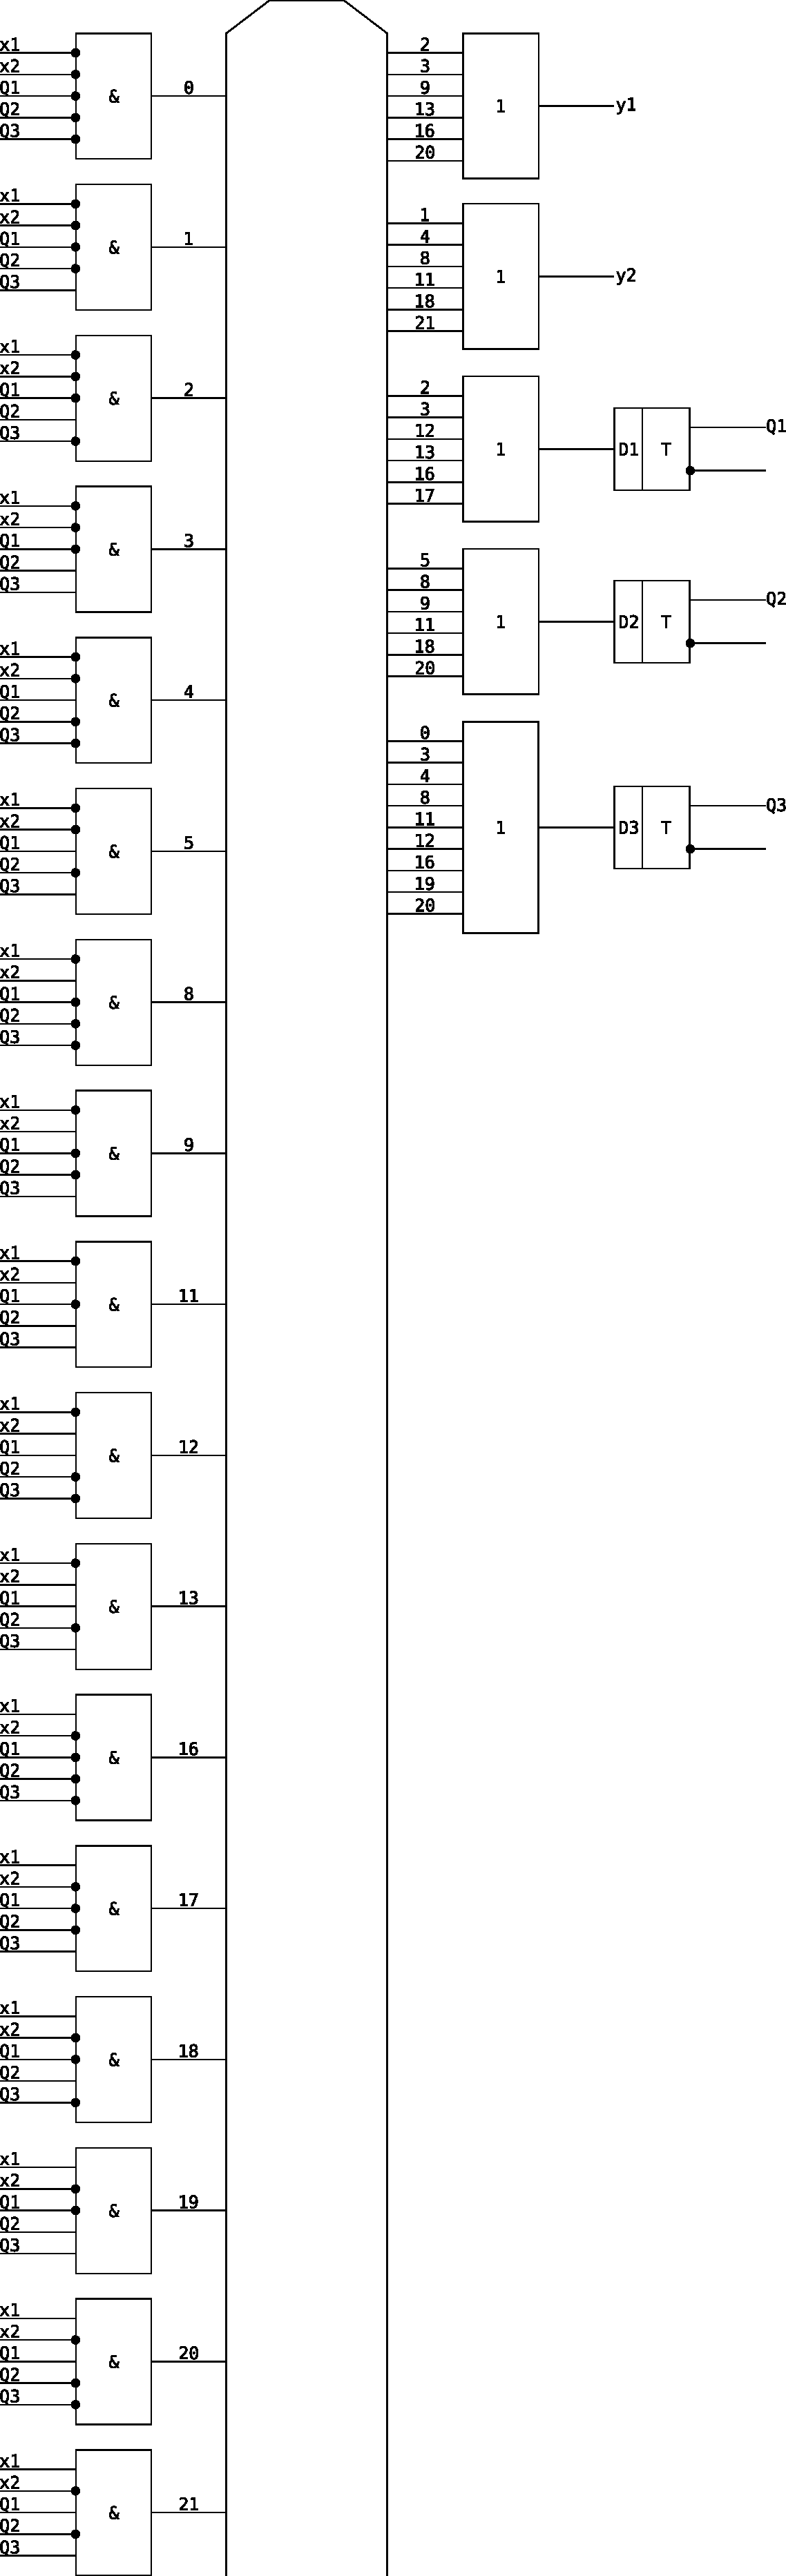
\includegraphics[width=0.44\textwidth]{sdffcircuit.pdf}
\restoregeometry

\subsection*{Проверка}

Проверим правильность работы функциональной схемы:

Входное слово (пары $x_1x_2$):

\verb|00 01 01 01 01 10 10 10 00 01 01 00 10 00 00 00 10 10|

Выходное слово (пары $y_1y_2$):

\verb|00 10 00 01 01 00 00 10 10 10 00 00 01 10 01 01 10 01|

Выходное слово совпадает с ожидаемым (см. анализ переходов)

\section*{Синтез автомата на T-триггерах}

С учетом закона функционирования T-триггера построим таблицу
сигналов функций возбуждения:

\begin{tabular}{|*{7}{c|}}
\hline
$x_1x_2/Q_1Q_2Q_3$ & 000 & 001 & 010 & 011 & 100 & 101\\\hline
00 & 001 & 001 & 110 & 110 & 101 & 111\\\hline
01 & 011 & 011 & 010 & 000 & 001 & 001\\\hline
10 & 101 & 101 & 000 & 010 & 111 & 101\\\hline
 & $T_1T_2T_3$ & $T_1T_2T_3$ & $T_1T_2T_3$ & $T_1T_2T_3$ & $T_1T_2T_3$ & $T_1T_2T_3$\\\hline
\end{tabular}

\begin{align*}
T_1 & = \bar{x_1}\bar{x_2}\bar{Q_1}Q_2\bar{Q_3} \lor \bar{x_1}\bar{x_2}\bar{Q_1}Q_2Q_3 \lor \bar{x_1}\bar{x_2}Q_1\bar{Q_2}\bar{Q_3} \lor \bar{x_1}\bar{x_2}Q_1\bar{Q_2}Q_3 \lor x_1\bar{x_2}\bar{Q_1}\bar{Q_2}\bar{Q_3} \lor x_1\bar{x_2}\bar{Q_1}\bar{Q_2}Q_3 \lor \\ & \lor x_1\bar{x_2}Q_1\bar{Q_2}\bar{Q_3} \lor x_1\bar{x_2}Q_1\bar{Q_2}Q_3 = \\ & = 2 \lor 3 \lor 4 \lor 5 \lor 16 \lor 17 \lor 20 \lor 21 \\
T_2 & = \bar{x_1}\bar{x_2}\bar{Q_1}Q_2\bar{Q_3} \lor \bar{x_1}\bar{x_2}\bar{Q_1}Q_2Q_3 \lor \bar{x_1}\bar{x_2}Q_1\bar{Q_2}Q_3 \lor \bar{x_1}x_2\bar{Q_1}\bar{Q_2}\bar{Q_3} \lor \bar{x_1}x_2\bar{Q_1}\bar{Q_2}Q_3 \lor \bar{x_1}x_2\bar{Q_1}Q_2\bar{Q_3} \lor \\ & \lor x_1\bar{x_2}\bar{Q_1}Q_2Q_3 \lor x_1\bar{x_2}Q_1\bar{Q_2}\bar{Q_3}   = \\ & = 2 \lor 3 \lor 5 \lor 8 \lor 9 \lor 10 \lor 19 \lor 20 \\
T_3 & = \bar{x_1}\bar{x_2}\bar{Q_1}\bar{Q_2}\bar{Q_3} \lor \bar{x_1}\bar{x_2}\bar{Q_1}\bar{Q_2}Q_3 \lor \bar{x_1}\bar{x_2}Q_1\bar{Q_2}\bar{Q_3} \lor \bar{x_1}\bar{x_2}Q_1\bar{Q_2}Q_3 \lor \bar{x_1}x_2\bar{Q_1}\bar{Q_2}\bar{Q_3} \lor \bar{x_1}x_2\bar{Q_1}\bar{Q_2}Q_3 \lor \\ & \lor \bar{x_1}x_2Q_1\bar{Q_2}\bar{Q_3} \lor \bar{x_1}x_2Q_1\bar{Q_2}Q_3 \lor x_1\bar{x_2}\bar{Q_1}\bar{Q_2}\bar{Q_3} \lor x_1\bar{x_2}\bar{Q_1}\bar{Q_2}Q_3 \lor x_1\bar{x_2}Q_1\bar{Q_2}\bar{Q_3} \lor x_1\bar{x_2}Q_1\bar{Q_2}Q_3 = \\ & = 0 \lor 1 \lor 4 \lor 5 \lor 8 \lor 9 \lor 12 \lor 13 \lor 16 \lor 17 \lor 20 \lor 21
\end{align*}

\subsection*{Функциональная схема}

\newpage
\newgeometry{top=1cm, bottom=1cm, left=1cm, right=1cm}
\thispagestyle{empty}
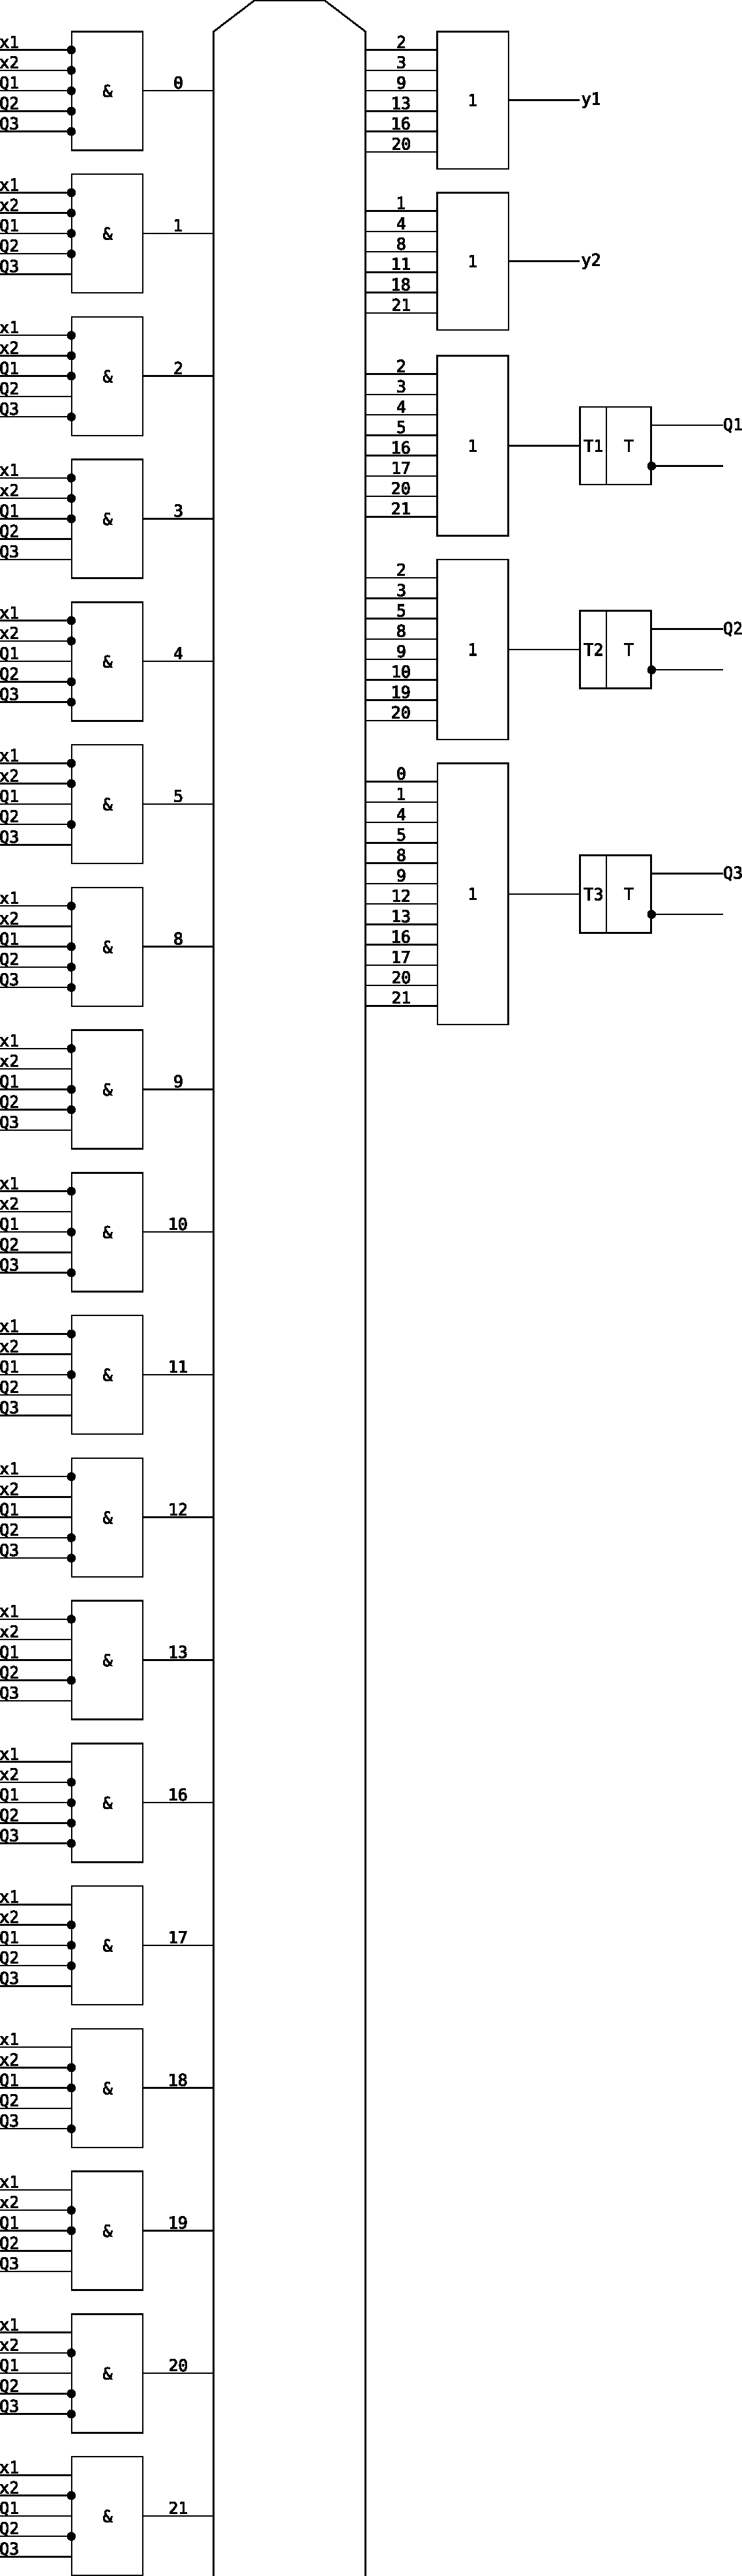
\includegraphics[width=0.41\textwidth]{stffcircuit.pdf}
\restoregeometry

\subsection*{Проверка}

Проверим правильность работы функциональной схемы:

Входное слово (пары $x_1x_2$):

\verb|00 01 01 01 01 10 10 10 00 01 01 00 10 00 00 00 10 10|

Выходное слово (пары $y_1y_2$):

\verb|00 10 00 01 01 00 00 10 10 10 00 00 01 10 01 01 10 01|

Выходное слово совпадает с ожидаемым (см. анализ переходов)

\section*{Синтез автомата на RS-триггерах}

С учетом закона функционирования RS-триггера построим таблицу
сигналов функций возбуждения:

\begin{tabular}{|c|*{6}{>{\centering\arraybackslash}p{2cm}|}}
\hline
$x_1x_2/Q_1Q_2Q_3$ & 000 & 001 & 010 & 011 & 100 & 101\\\hline
00 & -0/-0/01 & -0/-0/10 & 01/10/-0 & 01/10/0- & 10/-0/01 & 10/01/10\\\hline
01 & -0/01/01 & -0/01/10 & -0/10/-0 & -0/0-/0- & 0-/-0/01 & 0-/-0/10\\\hline
10 & 01/-0/01 & 01/-0/10 & -0/0-/-0 & -0/10/0- & 10/01/01 & 10/-0/10\\\hline
 & $R_1S_1$/ $R_2S_2$/ $R_3S_3\ $ & $R_1S_1$/ $R_2S_2$/ $R_3S_3\ $ & $R_1S_1$/ $R_2S_2$/ $R_3S_3\ $ & $R_1S_1$/ $R_2S_2$/ $R_3S_3\ $ & $R_1S_1$/ $R_2S_2$/ $R_3S_3\ $ & $R_1S_1$/ $R_2S_2$/ $R_3S_3\ $\\\hline
\end{tabular}

\begin{align*}
R_1 & = \bar{x_1}\bar{x_2}Q_1\bar{Q_2}\bar{Q_3} \lor \bar{x_1}\bar{x_2}Q_1\bar{Q_2}Q_3 \lor x_1\bar{x_2}Q_1\bar{Q_2}\bar{Q_3} \lor x_1\bar{x_2}Q_1\bar{Q_2}Q_3 = 4 \lor 5 \lor 20 \lor 21 \\
S_1 & = \bar{x_1}\bar{x_2}\bar{Q_1}Q_2\bar{Q_3} \lor \bar{x_1}\bar{x_2}\bar{Q_1}Q_2Q_3 \lor x_1\bar{x_2}\bar{Q_1}\bar{Q_2}\bar{Q_3} \lor x_1\bar{x_2}\bar{Q_1}\bar{Q_2}Q_3 = 2 \lor 3 \lor 16 \lor 17 \\
R_2 & = \bar{x_1}\bar{x_2}\bar{Q_1}Q_2\bar{Q_3} \lor \bar{x_1}\bar{x_2}\bar{Q_1}Q_2Q_3 \lor \bar{x_1}x_2\bar{Q_1}Q_2\bar{Q_3} \lor x_1\bar{x_2}\bar{Q_1}Q_2Q_3 = 2 \lor 3 \lor 10 \lor 19 \\
S_2 & = \bar{x_1}\bar{x_2}Q_1\bar{Q_2}Q_3 \lor \bar{x_1}x_2\bar{Q_1}\bar{Q_2}\bar{Q_3} \lor \bar{x_1}x_2\bar{Q_1}\bar{Q_2}Q_3 \lor x_1\bar{x_2}Q_1\bar{Q_2}\bar{Q_3} = 5 \lor 8 \lor 9 \lor 20 \\
R_3 & = \bar{x_1}\bar{x_2}\bar{Q_1}\bar{Q_2}Q_3 \lor \bar{x_1}\bar{x_2}Q_1\bar{Q_2}Q_3 \lor \bar{x_1}x_2\bar{Q_1}\bar{Q_2}Q_3 \lor \bar{x_1}x_2Q_1\bar{Q_2}Q_3 \lor x_1\bar{x_2}\bar{Q_1}\bar{Q_2}Q_3 \lor x_1\bar{x_2}Q_1\bar{Q_2}Q_3 = \\ & = 1 \lor 5 \lor 9 \lor 13 \lor 17 \lor 21 \\
S_3 & = \bar{x_1}\bar{x_2}\bar{Q_1}\bar{Q_2}\bar{Q_3} \lor \bar{x_1}\bar{x_2}Q_1\bar{Q_2}\bar{Q_3} \lor \bar{x_1}x_2\bar{Q_1}\bar{Q_2}\bar{Q_3} \lor \bar{x_1}x_2Q_1\bar{Q_2}\bar{Q_3} \lor x_1\bar{x_2}\bar{Q_1}\bar{Q_2}\bar{Q_3} \lor x_1\bar{x_2}Q_1\bar{Q_2}\bar{Q_3} = \\ & = 0 \lor 4 \lor 8 \lor 12 \lor 16 \lor 20
\end{align*}

\subsection*{Функциональная схема}

\newpage
\newgeometry{top=1cm, bottom=1cm, left=1cm, right=1cm}
\thispagestyle{empty}
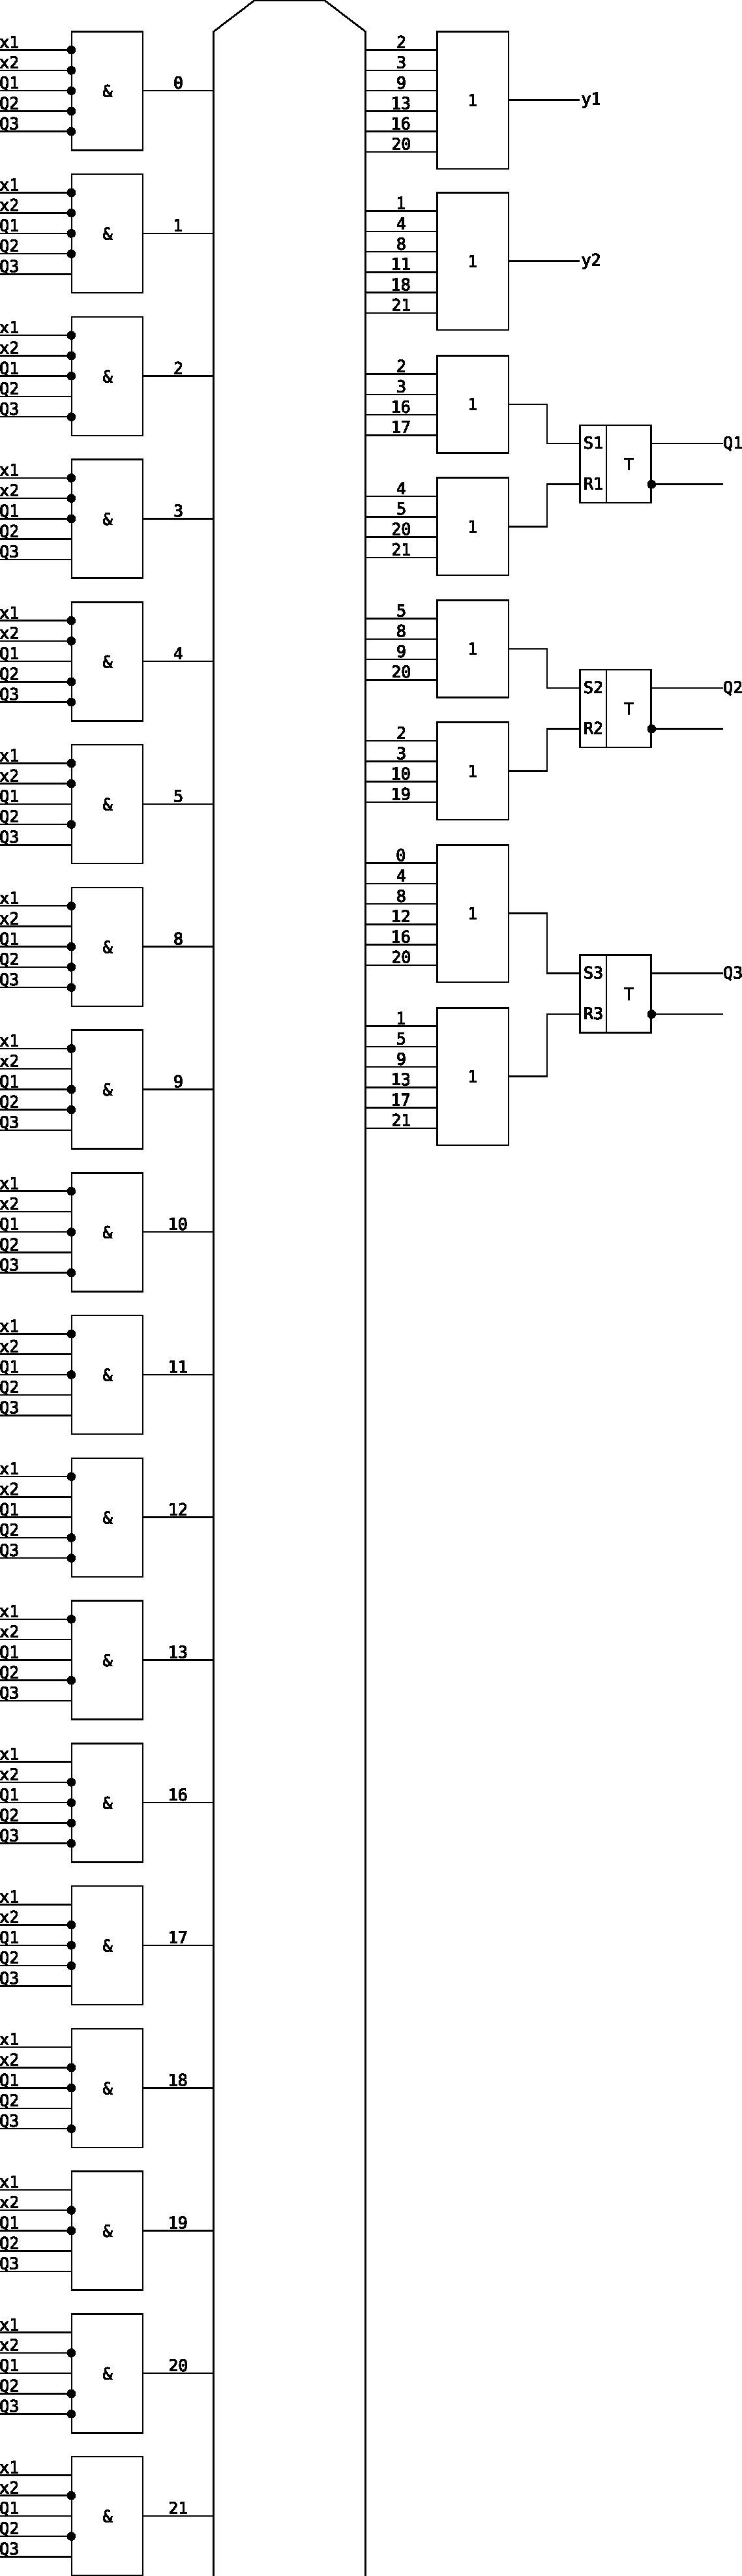
\includegraphics[width=0.41\textwidth]{srsffcircuit.pdf}
\restoregeometry

\subsection*{Проверка}

Проверим правильность работы функциональной схемы:

Входное слово (пары $x_1x_2$):

\verb|00 01 01 01 01 10 10 10 00 01 01 00 10 00 00 00 10 10|

Выходное слово (пары $y_1y_2$):

\verb|00 10 00 01 01 00 00 10 10 10 00 00 01 10 01 01 10 01|

Выходное слово совпадает с ожидаемым (см. анализ переходов)

\section*{Синтез автомата на JK-триггерах}

С учетом закона функционирования JK-триггера построим таблицу
сигналов функций возбуждения:

\begin{tabular}{|c|*{6}{>{\centering\arraybackslash}p{2cm}|}}
\hline
$x_1x_2/Q_1Q_2Q_3$ & 000 & 001 & 010 & 011 & 100 & 101\\\hline
00 & 0-/0-/1- & 0-/0-/-1 & 1-/-1/0- & 1-/-1/-0 & -1/0-/1- & -1/1-/-1\\\hline
01 & 0-/1-/1- & 0-/1-/-1 & 0-/-1/0- & 0-/-0/-0 & -0/0-/1- & -0/0-/-1\\\hline
10 & 1-/0-/1- & 1-/0-/-1 & 0-/-0/0- & 0-/-1/-0 & -1/1-/1- & -1/0-/-1\\\hline
 & $J_1K_1$/ $J_2K_2$/ $J_3K_3$ & $J_1K_1$/ $J_2K_2$/ $J_3K_3$ & $J_1K_1$/ $J_2K_2$/ $J_3K_3$ & $J_1K_1$/ $J_2K_2$/ $J_3K_3$ & $J_1K_1$/ $J_2K_2$/ $J_3K_3$ & $J_1K_1$/ $J_2K_2$/ $J_3K_3$\\\hline
\end{tabular}

\begin{align*}
J_1 & = \bar{x_1}\bar{x_2}\bar{Q_1}Q_2\bar{Q_3} \lor \bar{x_1}\bar{x_2}\bar{Q_1}Q_2Q_3 \lor x_1\bar{x_2}\bar{Q_1}\bar{Q_2}\bar{Q_3} \lor x_1\bar{x_2}\bar{Q_1}\bar{Q_2}Q_3 = 2 \lor 3 \lor 16 \lor 17 \\
K_1 & = \bar{x_1}\bar{x_2}Q_1\bar{Q_2}\bar{Q_3} \lor \bar{x_1}\bar{x_2}Q_1\bar{Q_2}Q_3 \lor x_1\bar{x_2}Q_1\bar{Q_2}\bar{Q_3} \lor x_1\bar{x_2}Q_1\bar{Q_2}Q_3 = 4 \lor 5 \lor 20 \lor 21 \\
J_2 & = \bar{x_1}\bar{x_2}Q_1\bar{Q_2}Q_3 \lor \bar{x_1}x_2\bar{Q_1}\bar{Q_2}\bar{Q_3} \lor \bar{x_1}x_2\bar{Q_1}\bar{Q_2}Q_3 \lor x_1\bar{x_2}Q_1\bar{Q_2}\bar{Q_3} = 5 \lor 8 \lor 9 \lor 20 \\
K_2 & = \bar{x_1}\bar{x_2}\bar{Q_1}Q_2\bar{Q_3} \lor \bar{x_1}\bar{x_2}\bar{Q_1}Q_2Q_3 \lor \bar{x_1}x_2\bar{Q_1}Q_2\bar{Q_3} \lor x_1\bar{x_2}\bar{Q_1}Q_2Q_3 = 2 \lor 3 \lor 10 \lor 19 \\
J_3 & = \bar{x_1}\bar{x_2}\bar{Q_1}\bar{Q_2}\bar{Q_3} \lor \bar{x_1}\bar{x_2}Q_1\bar{Q_2}\bar{Q_3} \lor \bar{x_1}x_2\bar{Q_1}\bar{Q_2}\bar{Q_3} \lor \bar{x_1}x_2Q_1\bar{Q_2}\bar{Q_3} \lor x_1\bar{x_2}\bar{Q_1}\bar{Q_2}\bar{Q_3} \lor x_1\bar{x_2}Q_1\bar{Q_2}\bar{Q_3} = \\ & = 0 \lor 4 \lor 8 \lor 12 \lor 16 \lor 20 \\
K_3 & = \bar{x_1}\bar{x_2}\bar{Q_1}\bar{Q_2}Q_3 \lor \bar{x_1}\bar{x_2}Q_1\bar{Q_2}Q_3 \lor \bar{x_1}x_2\bar{Q_1}\bar{Q_2}Q_3 \lor \bar{x_1}x_2Q_1\bar{Q_2}Q_3 \lor x_1\bar{x_2}\bar{Q_1}\bar{Q_2}Q_3 \lor x_1\bar{x_2}Q_1\bar{Q_2}Q_3 = \\ & = 1 \lor 5 \lor 9 \lor 13 \lor 17 \lor 21
\end{align*}

\subsection*{Функциональная схема}

\newpage
\newgeometry{top=1cm, bottom=1cm, left=1cm, right=1cm}
\thispagestyle{empty}
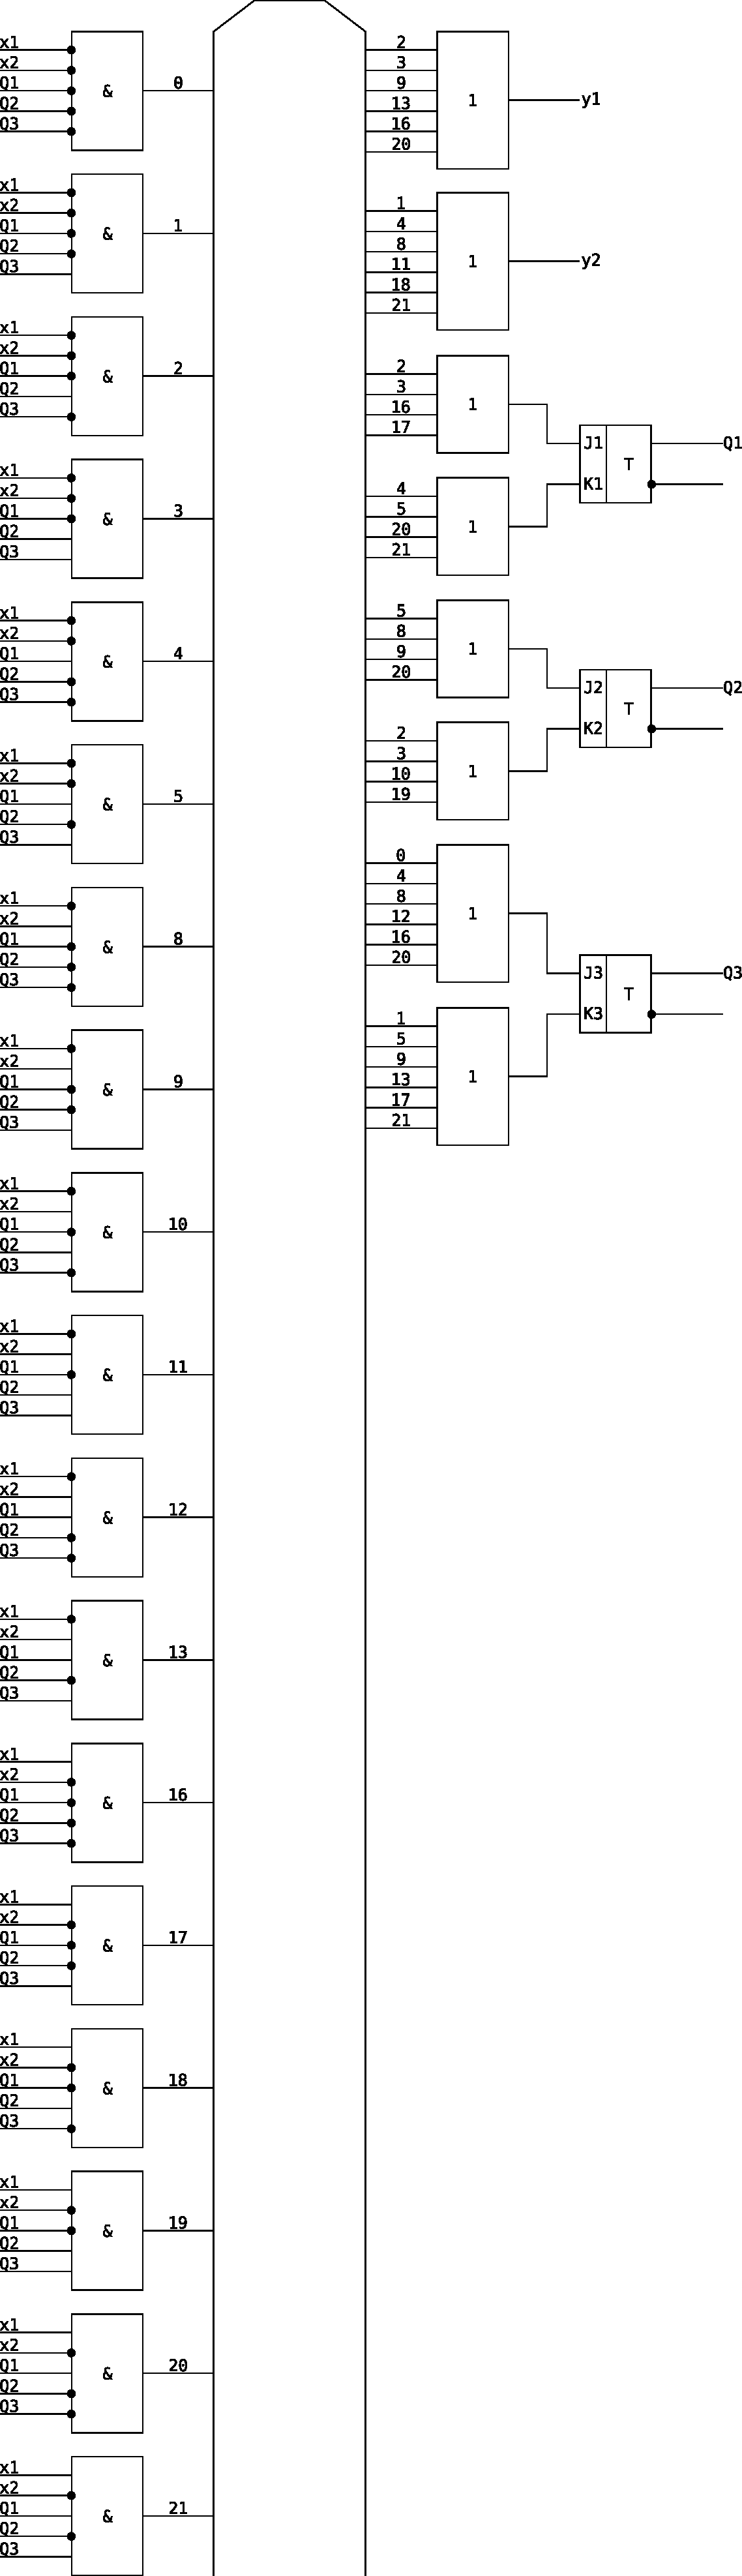
\includegraphics[width=0.41\textwidth]{sjkffcircuit.pdf}
\restoregeometry

\subsection*{Проверка}

Проверим правильность работы функциональной схемы:

Входное слово (пары $x_1x_2$):

\verb|00 01 01 01 01 10 10 10 00 01 01 00 10 00 00 00 10 10|

Выходное слово (пары $y_1y_2$):

\verb|00 10 00 01 01 00 00 10 10 10 00 00 01 10 01 01 10 01|

Выходное слово совпадает с ожидаемым (см. анализ переходов)

\section*{Вывод}

В ходе выполнения работы был изучен канонический метод структурного синтеза,
получены практические навыки преобразования абстрактного автомата Мили в
структурный автомат на D-, T-, RS- и JK-триггерах.

\end{document}
